\begin{alertblock}{Mutual Information Gain of Hop Patterns}
Mutual information gain measures the impact of hop patterns on semantic label distributions\\
\vspace{0.5cm}
{
\begin{column}{0.8\colwidth}
Analysis:
\begin{itemize}
    \item Hop pattern (0,1) has the highest information gain of 0.149bits
    \item Long hop patterns have near-zero information gains
    \item Short hop patterns have diverse non-zero information gains, ranging from 0.011 bits to 0.149bits
\end{itemize}
% \begin{itemize}
% % \vspace{0.8cm}
%     \item $X$: syntactic variable mapping predicate-argument pairs to their hop patterns
%     \begin{itemize}
%         \item $X_{(\alpha, \beta)}$: syntax-aware model sensitive to the hop pattern $X_{(\alpha, \beta)}$
%         \item $X_0$: syntax-agnostic model
%     \end{itemize}
%     \item $Y$: semantic variable mapping predicate-argument pairs to their semantic labels
        
%     \item $\Delta \mathrm{MI}(X_{(\alpha, \beta)}, X_0):=\mathrm{MI}(X_{(\alpha, \beta)}, Y) - \mathrm{MI}(X_0, Y)$
% \end{itemize}
\end{column}
\begin{column}{1.1\colwidth}
\begin{figure}
    \centering
    \captionsetup{justification=centering}
    \vspace{-1cm}
    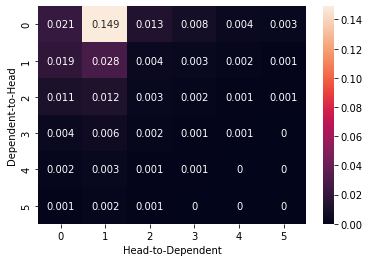
\includegraphics[width=0.75\textwidth]{images/ssdp-mi.png}
    \vspace{-0.5cm}
\caption{Mutual information gain of hop patterns up to (5, 5)}
    \label{fig:my_label}
\end{figure}
% \vspace{3cm}

\end{column}
}
\\
% {
%     \begin{align}
%     X_{(\alpha, \beta)}(p^s, a^s)&=\begin{cases}
%     1, (p^s, a^s)\text{ is of }(\alpha, \beta)\\
%     0, \text{otherwise}
%     \end{cases}\label{eq-rvsyn-aware}\\
%     X_0(p^s, a^s) &= 0\label{eq-rvsyn-agnostic}\\
%     \Delta \mathrm{MI}(X_{(\alpha, \beta)}, X_0) &= \mathrm{MI}(X_{(\alpha, \beta)}, Y) - \mathrm{MI}(X_0, Y) 
%     \label{eq-deltami}
%     \end{align}
% }
\vspace{-1.5cm}
{
\begin{column}{0.8\colwidth}
\begin{figure}
    \vspace{-3.2cm}
    % \RaggedLeft 
    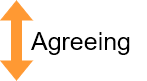
\includegraphics[width=0.3\textwidth]{images/agreement arrow.drawio.png}
    % \caption{Caption}
    % \label{fig:my_label}
\end{figure}
% \vspace{1cm}
Results:
\begin{itemize}
    \item Models assign a unique component to the hop pattern (0, 1), the hop pattern with the highest information gain
    \item Models assign long SSDPs with near-zero information gains to a single component
    \item Models assign SSDPs with diverse information gains to different components
\end{itemize}
\end{column}
% \separatorcolmun
\begin{column}{1.1\colwidth}
\begin{table}[]
\vspace{1cm}
\captionsetup{justification=centering}
\small
\centering
\begin{subtable}{0.3\textwidth}
\centering
\begin{tabular}{|l|r|r|r|r|} 
\hline
\backslashbox{$\alpha$}{$\beta$} & 0 & 1 & 2 & 3  \\ 
\hline
0 & \cellcolor{purple}3 & \cellcolor{white}1 & \cellcolor{gray}0 & \cellcolor{gray}0 \\ \hline
1 & \cellcolor{violet}2 & \cellcolor{violet}2 & \cellcolor{gray}0 & \cellcolor{gray}0 \\ \hline
2 & \cellcolor{violet}2 & \cellcolor{violet}2 & \cellcolor{gray}0 & \cellcolor{gray}0 \\ \hline
3 & \cellcolor{violet}2 & \cellcolor{gray}0 & \cellcolor{gray}0 & \cellcolor{gray}0 \\ \hline
4 & \cellcolor{gray}0 & \cellcolor{gray}0 & \cellcolor{gray}0 & \cellcolor{gray}0 \\ \hline
5 & \cellcolor{gray}0 & \cellcolor{gray}0 & \cellcolor{gray}0 & \cellcolor{gray}0 \\ \hline
\end{tabular}
% \vspace{0.5cm}
\subcaption{FastText}
% \label{tbl-cluster_assignment-glove}
\end{subtable}
\quad
\begin{subtable}{0.3\textwidth}
\centering
\begin{tabular}{|l|r|r|r|r|} 
\hline
\backslashbox{$\alpha$}{$\beta$} & 0 & 1 & 2 & 3  \\ 
\hline
0 & \cellcolor{purple}2 & \cellcolor{white}0 & \cellcolor{gray}4 & \cellcolor{gray}4 \\ \hline
1 & \cellcolor{purple}2 & \cellcolor{violet}1 & \cellcolor{gray}4 & \cellcolor{gray}4 \\ \hline
2 & \cellcolor{cyan}\cellcolor{cyan}3 & \cellcolor{cyan}3 & \cellcolor{gray}4 & \cellcolor{gray}4 \\ \hline
3 & \cellcolor{gray}4 & \cellcolor{gray}4 & \cellcolor{gray}4 & \cellcolor{gray}4 \\ \hline
4 & \cellcolor{gray}4 & \cellcolor{gray}4 & \cellcolor{gray}4 & \cellcolor{gray}4 \\ \hline
5 & \cellcolor{gray}4 & \cellcolor{gray}4 & \cellcolor{gray}4 & \cellcolor{gray}4 \\ \hline
\end{tabular}
% \vspace{0.5cm}
\subcaption{ELMo}
% \label{tbl-cluster_assignment-glove}
\end{subtable}
\quad
\begin{subtable}{0.3\textwidth}
\centering
\begin{tabular}{|l|r|r|r|r|}
\hline
\backslashbox{$\alpha$}{$\beta$} & 0 & 1 & 2 & 3 \\ \hline
0 & \cellcolor{purple}4 & \cellcolor{white}0 & \cellcolor{gray}2 & \cellcolor{gray}2 \\ \hline
1 & \cellcolor{purple}4 & \cellcolor{violet}3 & \cellcolor{gray}2 & \cellcolor{gray}2 \\ \hline
2 & \cellcolor{purple}4 & \cellcolor{violet}3 & \cellcolor{gray}2 & \cellcolor{gray}2 \\ \hline
3 & \cellcolor{purple}4 & \cellcolor{purple}4 & \cellcolor{gray}2 & \cellcolor{gray}2 \\ \hline
4 & \cellcolor{gray}2 & \cellcolor{gray}2 & \cellcolor{gray}2 & \cellcolor{gray}2 \\ \hline
5 & \cellcolor{gray}2 & \cellcolor{gray}2 & \cellcolor{gray}2 & \cellcolor{gray}2 \\ \hline
\end{tabular}
% \vspace{0.5cm}
\caption{BERT}
% \label{tbl-cluster_assignment-elmo}
\end{subtable}
\vspace{-0.5cm}
\caption{Component assignments extracted from models}
\label{tbl:cluster-assignment}
\end{table}
\end{column}
}

\textbf{Conclusion: \colorbox{yellow}{Semantic label distributions of different hop patterns have unique properties}}

\end{alertblock}